\chapter{Hierarquia de Classes}

    Um dos pontos fortes da programação orienta aos objetos diz respeito à compatibilidade de tipos, ou seja, para além de uma classe ser compatível com ela própria, é também compatível com outra qualquer, o que consequentemente permite uma certa abstração do tipo de dados.

    Tendo em conta que no futuro é expectável inserir novos tipos de artigos, podemos muito facilmente identificar uma pequena hierarquia de classes, na qual um \textit{Artigo} representa a superclasse e as suas especializações (\textit{Sapatilha, Mala} e \textit{Tshirt}) as respetivas subclasses, desta forma os artigos são tratados sem distinção pelos gestores, não havendo por isso a necessidade que estes conheçam em específico os dados que estão a manusear.

    \vspace{5pt}
    \begin{figure}[hb!]
        \centering
        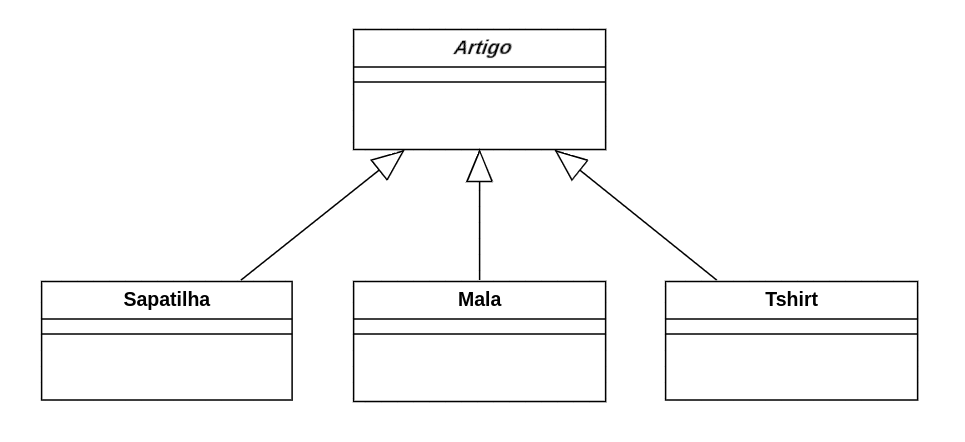
\includegraphics[width=0.7\textwidth]{imagens/11.png}
        \caption*{Figura 10. Hierarquia de classes}
    \end{figure}

    Uma vez que cada tipo de artigo possui uma fórmula de cálculo diferente, é necessário obrigar cada uma das subclasses a implementar um método conforme essas fórmulas, assim sendo é possível definir que a classe \textit{Artigo} é abstrata e que o método \textit{calculaPreço} também o é, pois consequentemente as subclasses são obrigadas a implementarem esse método. Desta forma criámos um certo polimorfismo, visto que ao invocar o método \textit{calculaPreço} na classe \textit{Artigo}, são utilizadas diferentes fórmulas sem que de facto nos apercebamos disso.

    Além disso, esta noção de hierarquia também apresenta várias vantagens ao nível da codificação, visto que as variáveis e métodos da classe \textit{Artigo} são herdados pelas subclasses, permitindo assim uma reutilização do código. 
    
    \section{Noção de Premium}

    O sistema deve ainda prever a existência de artigos e transportadoras \textit{premium,} o que a princípio parece ser facilmente resolvido através da implementação de uma interface, contudo não foi esta a decisão que tomámos.

    Quando dizemos que uma classe implementa uma determinada interface, estamos na verdade a dizer que essa classe segue um dado comportamento, assim sendo não faz qualquer sentido que a classe \textit{Artigo} ou \textit{Transportadora} implementem a interface \textit{Premium,} visto que existem artigos e transportadoras que não são \textit{premium}, e portanto não seguem esse comportamento já predefinido.

    Uma eventual forma de contornar este problema passaria pela criação de classes que especializassem \textit{Transportadora/Artigo} e fossem compatíveis com \textit{premium}, ou seja, criar algo como \textit{TransportadoraPremium, MalaPremium, SapatilhaPremium e TshirtPremium,} visto que desta forma as classes poderiam implementar \textit{Premium} sem qualquer problema de compatibilidade.

    Todavia esta solução parece um pouco rebuscada, e portanto resolvemos este problema da forma que nos pareceu mais adequada, ou seja, com a inserção de uma variável de instância (booleano) que define se um objeto segue a noção de \textit{premium.}